\documentclass[smaller,handout,table]{beamer}

\usetheme{clecturesty}

\subtitle{Lecture 2 of 5}

\begin{document}

{
\logo{
\includegraphics[width=0.30\textwidth]{imperialblue}}
\begin{frame}
  \titlepage
\end{frame}
}

\section{C Shorthand}
\subsection{Last Week...}
\begin{frame}{Last Week...}
\begin{itemize}
\item C is a language for creating fast, portable programs.
\item We use an IDE to write source, compile, link and debug our C programs.
\item The basic structure of a C program has been demonstrated and used.
\item There are two categories of number in C: integers and floating point numbers.
\item We have seen how logic and statements can control the flow of a program.
\item \texttt{printf} and \texttt{scanf} will write and read from the console respectively.
\end{itemize}
\end{frame}


\subsection{C Shorthand}
\begin{frame}[fragile]
\frametitle{Terse Code}
There are shortcuts in the C language that allow for concise code.
\begin{enumerate}
\item Incrementing by 1: Pre-increment, and post-increment.\\
\begin{tabular}{l l}
\tt ++i& Increment {\tt i} by 1, then use it.\\
\tt i++& Use {\tt i}, then increment it by 1.
\end{tabular}
\item Increment by another variable.\\
\begin{tabular}{r l}
Normal code:&\tt sum = sum + v[i];\\
Terse code:&\tt sum += v[i];
\end{tabular}
\end{enumerate}
An example:\\
\begin{semiverbatim}
   \kw{for} (i=0; i < N; i++)
      sum += v[i];
\end{semiverbatim}
\end{frame}

\begin{frame}
\frametitle{More Shorthand}
\begin{tabular}{l l}
\tt --i;&decrement {\tt i} by 1.\\
\tt sum -= v[i];&means {\tt sum = sum - v[i];}\\
\tt sum *= v[i];&means {\tt sum = sum * v[i];}\\
\tt sum /= v[i];&means {\tt sum = sum / v[i];}\\
\tt sum \%= 2;&means {\tt sum = sum \% 2;}
\end{tabular}\\
Other operators can also be abbreviated this way.
\begin{exampleblock}{Inline {\tt if} - The Ternary Operator}
The following code:\\
\texttt{\kw{if} (r1 > r2) \{ maxr = r1; \}\\
\kw{else} maxr = \{ r2; \} }\\
can be abbreviated:\\
\texttt{maxr = (r1 > r2) ? r1 : r2;}
\end{exampleblock}
\end{frame}



\section{Functions}

\subsection{Defining Functions}
\begin{frame}
\frametitle{Defining Functions}
The C language only provides essential functionality, meaning a lot of functions need to be written yourself. Here are a few general rules for functions:

\begin{itemize}
\item Functions cannot define other functions within them.
\item An optional single value can be returned.
\item All arguments to functions are passed by value and remain unaffected by the function.
\item Passing pointers to functions allows them to ``return'' multiple variables.
\end{itemize}
\end{frame}

\begin{frame}[fragile]
\frametitle{Declarations vs Definitions}
\begin{block}{Function Declarations}
These tell the compiler about the \emph{existence} of a function, which then
allows us to call it. A declaration ends with a {\tt ;}.
\begin{semiverbatim}
\kw{int} quad_roots (\kw{double} A, \kw{double} B, \kw{double} C,
                \kw{double} * r1, \kw{double} * r2);
\end{semiverbatim}
\end{block}

\begin{block}{Function Definitions}
The code making up the function is supplied to the compiler. A function can only be defined once. A definition contains braces {\tt \{} and {\tt \}}:
\begin{semiverbatim}
\kw{int} quad_roots (\kw{double} A, \kw{double} B, \kw{double} C,
                \kw{double} * r1, \kw{double} * r2)
\{...\}
\end{semiverbatim}
\end{block}
\end{frame}

\subsection{Using Functions}
\begin{frame}
\frametitle{An Example: Quadratic Equation Solver}
As a worked example we write a function to solve the quadratic equation:
$$ A x^2 + B x + C=0 \qquad A,B,C\in\mathbb{R}$$
Our quadratic solver will:
\begin{itemize}
\item Take the three doubles {\tt A}, {\tt B} and {\tt C} as arguments.
\item Solve the quadratic and return an \kw{\tt int} signifying to the caller the type of answer available:
\begin{tabular}{l l}
-1&{\tt A} = 0, we have a linear equation.\\
0&There are two distinct real roots.\\
1&We have a pair of complex conjugate roots.\\
2&Both roots are real and identical.
\end{tabular}
\end{itemize}
\end{frame}

\begin{frame}[fragile]
\frametitle{The Code}
One possible function prototype is:
\begin{semiverbatim}
\kw{int} quad_roots (\kw{double} A, \kw{double} B, \kw{double} C,
                \kw{double} * r1, \kw{double} * r2);
\end{semiverbatim}
\begin{itemize}
\item The variables {\tt A}, {\tt B} and {\tt C} are unchanged by {\tt quad\_roots}.
\item We need to return two doubles (the roots of the equation), thus we take in pointers {\tt \kw{double} *r1} and {\tt \kw{double} *r2}.
\item C90 does not allow for complex number types (C99 does support them), so we have to think a little bit about the complex number case.
\end{itemize}
\end{frame}

\begin{frame}[fragile]
\frametitle{Code Snippet for Calling {\tt quad\_roots}}
\begin{semiverbatim}
...
\kw{int} main()
\{
   \kw{double} A, B, C, root1, root2;
   \kw{int} quad_case;   
   ...   
   quad\_case = quad\_roots(A, B, C, \&root1,
                          \&root2);
                          
   \kw{switch}(quad\_case)
   \{
   \kw{case} -1: \emph{linear equation}
\end{semiverbatim}
\end{frame}

\begin{frame}[fragile]
\frametitle{Code Snippet for {\tt quad\_roots}}
\begin{semiverbatim}
\kw{int} quad\_roots(\kw{double} A, \kw{double} B, \kw{double} C,
               \kw{double} * r1, \kw{double} *r2)
\{
   \kw{double} d;
   
   \kc{/* linear case */}
   if (A == 0.0)
   \{
      *r1 = -C/B;
      \kw{return} -1;
   \}
          
   \kc{/* compute the discriminant */}
   d = B*B-4.0*A*C;
\end{semiverbatim}
\end{frame}

\subsection{Structuring Functions}
\begin{frame}[fragile]
\frametitle{The Stack}
Let's consider this example function.
\begin{columns}
\begin{column}{5cm}
\begin{semiverbatim}
\kw{int} hasRealRoots(\alert<2>{\kw{double} A},
       \alert<2>{\kw{double} B, \kw{double} C})
\{
   \alert<3>{\kw{double} d} = B*B-4.0*A*C;
   \kw{if} (d < 0) \alert<4>{\kw{return}} 0;
   \alert<4>{\kw{return}} 1;
\}
\end{semiverbatim}
\end{column}
\begin{column}{5cm}
\begin{itemize}
\alert<2>{\item We need space to hold a copy of {\tt A}, {\tt B} and {\tt C}.} 
\alert<3>{\item We need space to store our computed {\tt d}.}
\alert<4>{\item When we've finished, we need to get back to the calling function.}
\end{itemize}
\end{column}
\end{columns}
\vspace{0.1in}
\begin{block}<5>{}
\begin{center}
\alert<5>{This is achieved by using a \emph{stack}.}
\end{center}
\end{block}
\end{frame}

\begin{frame}
\frametitle{The Stack - Rough Sketch (Stack Frames)}
\begin{columns}
\begin{column}{5cm}
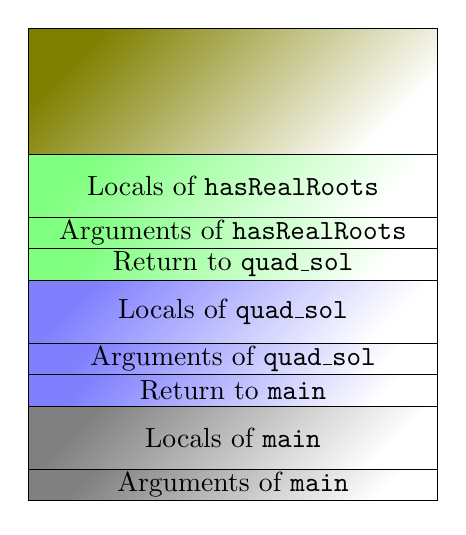
\begin{tikzpicture}[]
\shadedraw [shading angle=45] (0,0) rectangle +(5.2,0.4);
\node at (2.6,0.2) {Arguments of \tt main};
\shadedraw [shading angle=45] (0,0.4) rectangle +(5.2,0.8);
\node at (2.6,0.8) {Locals of \tt main};
\shadedraw [top color=blue!50,shading angle=45] (0,1.2) rectangle +(5.2,0.4);
\node at (2.6,1.4) {Return to \tt main};
\shadedraw [top color=blue!50,shading angle=45] (0,1.6) rectangle +(5.2,0.4);
\node at (2.6,1.8) {Arguments of \tt quad\_sol};
\shadedraw [top color=blue!50,shading angle=45] (0,2.0) rectangle +(5.2,0.8);
\node at (2.6,2.4) {Locals of \tt quad\_sol};
\shadedraw [top color=green!50,shading angle=45] (0,2.8) rectangle +(5.2,0.4);
\node at (2.6,3.0) {Return to \tt quad\_sol};
\shadedraw [top color=green!50,shading angle=45] (0,3.2) rectangle +(5.2,0.4);
\node at (2.6,3.4) {Arguments of \tt hasRealRoots};
\shadedraw [top color=green!50,shading angle=45] (0,3.6) rectangle +(5.2,0.8);
\node at (2.6,4.0) {Locals of \tt hasRealRoots};
\shadedraw [top color=green!50!red,shading angle=45] (0,4.4) rectangle +(5.2,1.6);
\end{tikzpicture}
\end{column}
\begin{column}{6cm}
\begin{itemize}
\item Consider the case where we have {\tt main}, which calls \textcolor{blue}{\tt quad\_sol}, which in turn calls \textcolor{green}{\tt hasRealRoots}.
\item We add and remove items from the stack as the program executes.
\item Adding/removing items from the stack takes very little time.
\item The stack is fixed in size, if we go over the top (``smash the stack'')
, our program crashes.
\end{itemize}
\end{column}
\end{columns}
\end{frame}

\begin{frame}
\frametitle{Recursive Functions}
As C uses a stack by default when calling functions, we are able to write functions that call themselves. These are called \emph{recursive functions}.

\begin{block}{An Example: Computing the Factorial}
$$n! = \prod_{i=1}^n i,  \quad 0! = 1, \qquad n\in\mathbb{N}.$$
Lends itself to be coded up as a recursive function.
\end{block}

\begin{block}{A Tougher Example: Fibonacci Numbers}
$$ F_n = F_{n-1} + F_{n-2}, \qquad F_0 = F_1 = 1.$$
A na\"ive implementation of this will kill the stack, and take a very long time to execute.
\end{block}
\end{frame}

\begin{frame}[fragile]
\frametitle{Computing the Factorial}
\begin{semiverbatim}
\kr\kl\kw{\#include} \kt{<stdio.h>}
\kl
\kl\kw{int} NFact(\kw{int} N)
\kl\{
\kl   \kw{if} (N>1) \kw{return} N*NFact(N-1);
\kl   \kw{return} 1;
\kl\}
\kl
\kl\kw{int} main()
\kl\{
\kl   \kw{int} n;
\kl   printf(\kt{"Enter n:"});
\kl   scanf(\kt{"%d"}, &n);
\kl   printf(\kt{"%d! = %d\\n"}, n, NFact(n));
\kl   \kw{return} 0;
\kl\}
\end{semiverbatim}
\end{frame}

\begin{frame}[fragile]
\frametitle{Computing Fibonacci Numbers}
\begin{columns}
\begin{column}{6cm}
\begin{alertblock}{}
\begin{semiverbatim}
\kw{int} BadFib(\kw{int} N)
\{
   \kw{if} (N < 2) \kw{return} 1;
   \kw{return} (BadFib(N-1) +
           BadFib(N-2));
\}
\end{semiverbatim}
\end{alertblock}
\end{column}
\begin{column}{3cm}
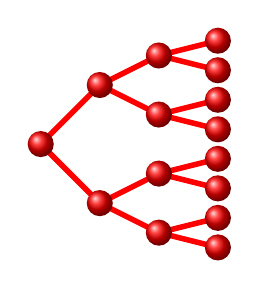
\begin{tikzpicture}[scale=0.75]
\tikzstyle{every node}=[ball color=red,circle,text=white]
\tikzstyle{edge from parent}=[draw,dashed,thick,red]
\draw[line width=2pt,color=red] (0,0) -- (1.0,1.0);
\draw[line width=2pt,color=red] (0,0) -- (1.0,-1.0);
\draw[line width=2pt,color=red] (1.0,1.0) -- (2.0,1.5);
\draw[line width=2pt,color=red] (1.0,1.0) -- (2.0,0.5);
\draw[line width=2pt,color=red] (1.0,-1.0) -- (2.0,-0.5);
\draw[line width=2pt,color=red] (1.0,-1.0) -- (2.0,-1.5);
\draw[line width=2pt,color=red] (2.0,1.5) -- (3.0,1.75);
\draw[line width=2pt,color=red] (2.0,1.5) -- (3.0,1.25);
\draw[line width=2pt,color=red] (2.0,0.5) -- (3.0,0.75);
\draw[line width=2pt,color=red] (2.0,0.5) -- (3.0,0.25);
\draw[line width=2pt,color=red] (2.0,-0.5) -- (3.0,-0.25);
\draw[line width=2pt,color=red] (2.0,-0.5) -- (3.0,-0.75);
\draw[line width=2pt,color=red] (2.0,-1.5) -- (3.0,-1.75);
\draw[line width=2pt,color=red] (2.0,-1.5) -- (3.0,-1.25);
\node at (0,0) {};
\node at (1.0, 1.0) {};
\node at (1.0, -1.0) {};
\node at (2.0, 1.5) {};
\node at (2.0, 0.5) {};
\node at (2.0, -0.5) {};
\node at (2.0, -1.5) {};
\node at (3.0, 1.75) {};
\node at (3.0, 1.25) {};
\node at (3.0, 0.75) {};
\node at (3.0, 0.25) {};
\node at (3.0, -0.75) {};
\node at (3.0, -0.25) {};
\node at (3.0, -1.75) {};
\node at (3.0, -1.25) {};
\end{tikzpicture}
\end{column}
\end{columns}

\begin{columns}
\begin{column}{7cm}
\begin{exampleblock}{}
\begin{semiverbatim}
\kw{int} utilf(\kw{int} a, \kw{int} b, \kw{int} n)
\{
   \kw{if}(n < 1) \kw{return} b;
   \kw{return} utilf(b, a+b, n-1);
\}
\kw{int} GoodFib(\kw{int} n)
\{
   \kw{return} utilf(0, 1, n);
\}
\end{semiverbatim}
\end{exampleblock}
\end{column}
\begin{column}{3cm}
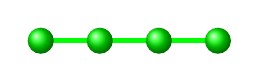
\begin{tikzpicture}[scale=0.75]
\tikzstyle{every node}=[ball color=green,circle,text=white]
\tikzstyle{edge from parent}=[draw,dashed,thick,green]
\draw[line width=2pt,color=green] (0,0) -- (1.0,0.0) -- (2.0, 0.0) -- (3.0, 0.0);
\node at (0,0) {};
\node at (1,0) {};
\node at (2,0) {};
\node at (3,0) {};
\end{tikzpicture}
\end{column}
\end{columns}
\end{frame}

\subsection{Code Structure}
\begin{frame}
\frametitle{Imperative versus Functional Programming}
Two programming techniques are popular in C:
\begin{alertblock}{Imperative}
\begin{itemize}
\item Very long functions.
\item Lots of global variables.
\item Very few function calls.
\end{itemize}
\end{alertblock}

\begin{exampleblock}{Functional}
\begin{itemize}
\item Lots of small functions.
\item Each function has a clearly defined r\^ole.
\item Global variables avoided as much as possible.
\end{itemize}
\end{exampleblock}
I would encourage leaning towards the latter, a good program will contain traits from both styles.
\end{frame}


\begin{frame}
\frametitle{Functions with Variable Number of Arguments}
Sometimes we don't know in advance how many arguments (or what type) a function needs, so C allows functions to have an unknown number of arguments. Two examples we've seen so far are {\tt printf} and {\tt scanf}.

\begin{itemize}
\item The first parameter must be of a normal type (i.e. \kw{\tt int}).
\item Three dots ({\tt ...}) are used for the last parameter.
\end{itemize}
\begin{center}
{\tt \kw{int} printf(\kw{char} * formatString, ...)}
\end{center}
\begin{block}{Handling variable arguments}
Variable arguments are manipulated using {\tt va\_start()}, {\tt va\_arg()},
and {\tt va\_end()}. These are found in \kt{\tt <stdarg.h>}.
\end{block}

\begin{alertblock}{}
Having just introduced these, I'm going to ask you {\bf not} to use them! Arrays are almost always more appropriate to use.
\end{alertblock}
\end{frame}


\subsection{Handling the Command Line}
\begin{frame}[fragile]
\frametitle{Handling the command-line in C}
\begin{itemize}
\item So far, we have used the prototype: {\tt \kw{int} main(\kw{void})}.
\item UNIX and Windows support command-line arguments to programs, and these need to be passed to main somehow.
\item There is another prototype of {\tt main} we are allowed to use:\\
\begin{center}
\tt \kw{int} main(\kw{int} argc, \kw{char} ** argv)
\end{center}
\end{itemize}
The example below prints out the command-line arguments to a program:
\vspace{-0.1in}
\begin{semiverbatim}
\small
\kw{\#include} \kt{<stdio.h>}

\kw{int} main(\kw{int} argc, \kw{char} ** argv)
\{
   \kw{int} loop;
   \kw{for} (loop = 0; loop < argc; loop++)
      printf(\kt{"argv[\%d] = \%s\\n"}, loop, argv[loop]);
   \kw{return} 0;
\}
\end{semiverbatim}
\end{frame}


\subsection{Functions - Summary}
\begin{frame}
\frametitle{Functions - Summary}
\begin{itemize}
\item Functions need to be declared before they are used. This is often done in \emph{header files}.
\item Up to one value can be returned from a function using the \kw{\tt return} statement.
\item A variable {\tt var} can be changed by a function if we pass the pointer
{\tt \&var}.
\item Pointers are declared using {\tt type * variable;}
\end{itemize}
\end{frame}

\section{Arrays}
\subsection{Data Arrays}
\begin{frame}
\frametitle{Arrays}
\begin{itemize}
\item These are blocks of data, all of the same type. Each element is indexed
using the array index operator:\\
e.g. {\tt myArray[index]} or {\tt primes[3]}.
\item Arrays are declared with types and sizes:\\
e.g. {\tt \kw{double} xVector[3];}
\item Arrays can be initialised:\\
e.g. {\tt \kw{int} primes[6] = \{2, 3, 5, 7, 11, 13\};}
\item All the elements of an array can be initialised to the \emph{same} value:
e.g. {\tt \kw{double} lotsOfDoubles[100] = \{0.0\};}
\item \bf Arrays in C are indexed from 0!
\end{itemize}
\end{frame}

\begin{frame}[fragile]
\frametitle{Accessing Array Elements}
\begin{alertblock}{}
\begin{center}
\bf Arrays in C are indexed from 0!
\end{center}
\end{alertblock}
\begin{semiverbatim}
\kw{\#include} \kt{<stdio.h>}

\kw{int} main()
\{
   \kw{int} primes[6] = \{2, 3, 5, 7, 11, 13\};

   printf(\kt{"first prime = \%d\\n"}, primes[0]);
   printf(\kt{"next prime = \%d\\n"}, primes[1]);
   
   \kw{return} 0;   
\}
\end{semiverbatim}
\end{frame}

\subsection{A Little More on Pointers}
\begin{frame}
\frametitle{A little more on pointers}
\begin{block}{Reminder}
\begin{itemize}
\item Declared using: {\tt type * ptrVar;}
\item Variable to pointer (pointer \emph{referencing}): {\tt ptrA = \&A;}
\item Pointer to variable (pointer \emph{de-referencing}):\\ {\tt *ptrA = newVar;}
\end{itemize}
\end{block}
\begin{exampleblock}{In addition}
Pointers are memory addresses, and as such allow arithmetic!
\end{exampleblock}
\end{frame}

\begin{frame}[fragile]
\frametitle{Pointer Arithmetic}
\begin{itemize}
\item Different data types in C are different sizes.
\item Pointers are usually declared with a type (i.e. {\tt \kw{int} *},
{\tt \kw{float} *}, {\tt \kw{double} *}).

\begin{alertblock}{Relation to Arrays}
Given the array {\tt myArray} and an integer {\tt index}, the following is true:
\begin{center}
\tt myArray[index] = *(myArray + index)
\end{center}
\end{alertblock}

\item And this is the reason array indices start at 0...
\end{itemize}

\end{frame}

\section{Debugging}
\subsection{Debugging Techniques}
\begin{frame}
\frametitle{Debugging}
\begin{itemize}
\item Once you've designed, typed up and successfully compiled your program, the difficult part begins: debugging!
\item Problems in the code are usually either easy to locate or stubbornly elusive.
\end{itemize}

\begin{exampleblock}{Easier Problems}
\begin{itemize}
\item Program crash/fault at the same point every run.
\end{itemize}
\end{exampleblock}

\begin{alertblock}{Nastier Problems}
\begin{itemize}
\item Numerical output differs to what is expected.
\item Program crashes seemingly randomly.
\end{itemize}
\end{alertblock}
\end{frame}

\begin{frame}
\frametitle{Debugging Techniques}
{\footnotesize
In increasing order of difficulty:
\begin{block}{Create Verbose Output}
\begin{itemize}
\item A few strategically placed {\tt printf} statements can prove to be helpful, but they have to be read (by a human):
\begin{itemize}
\item too few and you miss the problem,
\item too many and they rapidly become useless.
\end{itemize}
\item Straightforward to implement (and to comment out).
\end{itemize}
\end{block}

\begin{block}{Code Defensively}
\begin{itemize}
\item Consider specialised test cases.
\item Write code to test intermediate results.
\item Use the {\tt assert} macro.
\end{itemize}
\end{block}

\begin{block}{Use a Debugger}
For those non-trivial problems.
\end{block}
}
\end{frame}

\subsection{Assertion Checking}
\begin{frame}
\frametitle{Assertion Checking}
In the header \kt{\tt <assert.h>}, the macro {\tt assert} is defined. It has the following syntax:\\
\begin{center}
\tt assert(\emph{logical\_expression});
\end{center}
If \emph{logical\_expression} evaluates to false (zero) then:
\begin{itemize}
\item Program execution stops immediately.
\item An error message is sent to \emph{stderr} (the console) stating the line number where the assertion failed.
\end{itemize} 
\begin{block}{}
{\tt assert( a != 0); \kc{/* a should never be zero */}}
\end{block}
\begin{exampleblock}{Switching it off}
Placing {\tt \kw{\#define} NDEBUG} before all the \mbox{\tt \kw{\#include} \kt{<assert.h>}}
statements de-activates assertion checking.
\end{exampleblock}
\end{frame}

\begin{frame}[fragile]
\frametitle{Assertion Checking - An Example}
\vspace{-0.2in}
\begin{semiverbatim}
\scriptsize
\kr\kl\kw{\#include} \kt{<stdio.h>}
\kl\kw{\#include} \kt{<assert.h>}
\kl\kc{/* the sqrt function is much better than this... */}
\kl\kw{double} squareRoot(\kw{double} N)
\kl\{
\kl   \kw{double} x = 1.0;
\kl   \kw{int} loop;
\kl   \kc{/* negative numbers are not allowed! */}
\kl   assert(N >= 0.0);
\kl   \kw{if} (N == 0.0) \kw{return} 0.0;
\kl   \kw{for} (loop = 0; loop < 10; loop++)
\kl      x = (x*x+N)/(2.0*x);
\kl   \kw{return} x;
\kl\}
\kl
\kl\kw{int} main()
\kl\{
\kl   \kw{double} square;
\kl   printf(\kt{"Enter a non-negative number:"});
\kl   scanf(\kt{"\%lg"}, \&square);
\kl   \kc{/* SHOULD HAVE: if (x < 0.0) ...        */}
\kl   printf(\kt{"Square root = \%g\\n"}, squareRoot(square));
\kl   \kw{return} 0;
\kl\}
\end{semiverbatim}
\end{frame}

\subsection{Compile-time Logic}
\begin{frame}[fragile]
\frametitle{The C Preprocessor - Conditional Compilation}
We have already seen the {\tt \kw{\#include}} and {\tt \kw{\#define}} statements. Conditional statements are also possible:
\vspace{-0.2in}
\begin{semiverbatim}
\small
\kr\kl\kw{\#include} \kt{<stdio.h>}
\kl
\kl\kw{int} main(\kw{int} argc, \kw{char} ** argv)
\kl\{
\kl\kw{\#ifdef} NDEBUG
\kl   printf(\kt{"Assertions DISABLED\\n"});
\kl   printf(\kt{"\%d arguments\\n"}, argc);
\kl\kw{\#else}
\kl   printf(\kt{"Assertions ENABLED\\n"});
\kl\kw{\#endif}
\kl   \kw{return} 0;
\kl\}
\end{semiverbatim}
\begin{alertblock}{}
This logic is performed at \emph{compile time}.
\end{alertblock}
\end{frame}

\subsection{Using a Debugger}
\begin{frame}
\frametitle{Using a Debugger}
\begin{itemize}
\item Microsoft's Visual Studio contains a brilliant interactive debugger.
\item GNU debugger ({\tt gdb}) is also very good, and is essential for certain scenarios.
\item Programs need to be compiled with debug information.
\item Running a program straight through a debugger will show you the line of code that crashed it (if it crashes).
\end{itemize}

\begin{exampleblock}{Interactive Analysis of Running Code}
\begin{itemize}
\item Program execution can be paused at \emph{breakpoints}.
\item Functions can be \emph{stepped into}, \emph{stepped over}, or
\emph{stepped out from}.
\item Variables/arrays can be \emph{watched}.
\end{itemize}
\end{exampleblock}

\begin{alertblock}{}
Interactive debugging is very tricky at first, but soon becomes invaluable for isolating subtle problems.
\end{alertblock}
\end{frame}


\section{Causes of Error}

\subsection{Maths}
\begin{frame}
\frametitle{Common Problems}
\begin{enumerate}
\item Misuse of Power!\\
$x^2$ should always be written {\tt x*x}, \emph{NOT} {\tt pow(x, 2.0)}.\\
$\sqrt{x}$ should be written {\tt sqrt(x)}, \emph{NOT} {\tt pow(x, 0.5)}.
\item Integer Division\\
Remember a fraction such as {\tt 1/3} is equal to zero. To get a floating point fraction, this should be rewritten {\tt 1.0/3.0}.
\end{enumerate}
\end{frame}

\subsection{Floating Point Numbers}
\begin{frame}
\frametitle{Floating Point Numbers (IEEE 754 Standard)}
\framesubtitle{(from the previous lecture)}
On my machine, a \kw{\tt float} (single precision) looks like:\\
\begin{center}
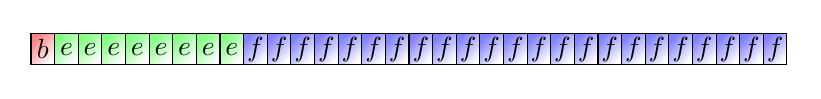
\begin{tikzpicture}[]
\shadedraw [top color=red!50,shading angle=45] (0,0) rectangle +(0.3,0.4);
\node at (0.15,0.2) {$b$};
\foreach \x in {0.3, 0.6, ..., 2.7}
   \shadedraw [top color=green!50,shading angle=45] (\x,0) rectangle +(0.3,0.4);

\foreach \x in {0.45, 0.75, ..., 2.85}
   \node at (\x,0.2) {$e$};
   
\foreach \x in {2.7, 3.0, ..., 9.6}
   \shadedraw [top color=blue!50,shading angle=45] (\x,0) rectangle +(0.3,0.4);
   
\foreach \x in {2.85, 3.15, ..., 9.45}   
   \node at (\x,0.2) {$f$};
\end{tikzpicture}
\end{center}
It consists of three parts, the \textcolor{red}{\emph{sign bit}$(b)$}, the \textcolor{green}{\emph{biased exponent}$(e)$} and the \textcolor{blue}{\emph{fraction}$(f)$}.
We break down a number $x$:
$$x^{\textrm{float}} = \textcolor{red}{(-1)^b} \times 
\textcolor{green}{2^{e-127}} \times \textcolor{blue}{\left(1+f\times2^{-23}\right)},
\begin{array}{c}
0 < e < 255\\0 \leq f \leq 2^{23}-1
\end{array},$$
We have three special numbers, {\tt -Inf} ($-\infty$), {\tt Inf} ($\infty$) and {\tt NaN} (Not a Number).

For \kw{\tt double} (double precision) we have:
$$x^{\textrm{double}} = (-1)^b\times 2^{e-1023}\times\left(1+f\times2^{-52}\right),
\begin{array}{c}
0 < e < 2047\\0 \leq f \leq 2^{52}-1
\end{array}.$$
\end{frame}

\begin{frame}
\frametitle{Floating Point Number Analysis}
In \kt{\tt <float.h>}, there are some useful quantities:
\resizebox{\textwidth}{!}{
\rowcolors[]{1}{blue!20}{blue!10}
\begin{tabular}{l l l}
\bf Quantity&\bf Float&\bf Double\\
Maximum Value&\tt FLT\_MAX&\tt DBL\_MAX\\
Minimum Value&\tt FLT\_MIN&\tt DBL\_MIN\\
Max Decimal Exponent&\tt FLT\_MAX\_10\_EXP&\tt DBL\_MAX\_10\_EXP\\
Min Decimal Exponent&\tt FLT\_MIN\_10\_EXP&\tt DBL\_MIN\_10\_EXP\\
$\epsilon$&\tt FLT\_EPSILON&\tt DBL\_EPSILON
\end{tabular}}

\begin{block}{Floating point $\epsilon$}
$\epsilon$ is the smallest (in magnitude) number such that:\\
\begin{center}
{\tt 1.0+$\epsilon$ != 1.0}
\end{center}
\end{block}
\end{frame}

\begin{frame}
\frametitle{Floating Point Accuracy}
\begin{itemize}
\item Some numbers can be represented in floating point exactly:
e.g. $2^i$, any integers that fit in the significand (mantissa).
\item Most numbers need to be approximated, e.g. $\sqrt{2}$, $\pi$.
\item One overlooked example is {\tt0.1}!
\item It is possible (though rare) to get exact answers from floating point arithmetic
\item Relative errors of $\approx10^{-15}$ for \kw{\tt double} and
$\approx10^{-6}$ for \kw{\tt float} are considered to be very good.
\item Multiplication and division generally preserve relative error (but can take us outside the floating point range).
\end{itemize}
\end{frame}

\begin{frame}
\frametitle{The Largest Source of Floating Point Errors}
Addition and subtraction are the largest contributors to floating point error.

\begin{alertblock}{The Golden Rule}
{\bf Do not subtract two very similar floating point numbers!}
\end{alertblock}

(This leads to ``\emph{catastrophic cancellation}''.)
\end{frame}

\subsection{Casting}
\begin{frame}[fragile]
\frametitle{Casting}
Casting can either be \emph{implicit} or \emph{explicit}.
\begin{block}{Implicit Casting}
Conversion where there is no ambiguity (i.e. to a ``bigger'' data type) can be done automatically:
\begin{semiverbatim}
\small\kw{double} x = 5; \kc{/* conversion from int to double */}
\kw{double} fEps = FLT\_EPSILON; \kc{/* float to double */}
\end{semiverbatim}
\end{block}

\begin{block}{Explicit Casting}
If we wish to force a type conversion we place the destination type in brackets before the source variable:
\begin{semiverbatim}
oldtype oldData = ...
newtype newData = (newtype) oldData;
\end{semiverbatim}
Explicit casting should be avoided if possible.
\end{block}
\end{frame}


\subsection{Precedence}
\begin{frame}
\frametitle{Operator Precedence and Associativity}
\framesubtitle{From K\&R2:}
\begin{columns}
\begin{column}{9cm}
\resizebox{\textwidth}{!}{
\begin{tabular}{l| l}
Operators&Associativity\\
\hline
\tt () [] -> .&left to right\\
\tt ! $\sim$ ++ -- + - * \& (\emph{type}) \kw{sizeof}&right to left\\
\tt * / \%&left to right\\
\tt + -&left to right\\
\tt << >>&left to right\\
\tt < <= > >=&left to right\\
\tt == !=&left to right\\
\tt \&&left to right\\
\tt \^&left to right\\
\tt |&left to right\\
\tt \&\&&left to right\\
\tt ||&left to right\\
\tt ?:&right to left\\
\tt = += -= *= /= \%= \&= $\wedge$= |= $\ll$= $\gg$=&right to left\\
\tt ,&left to right
\end{tabular}}
\end{column}
\end{columns}
\end{frame}

\begin{frame}
\frametitle{Operator Precedence and Associativity - Examples}
\begin{exampleblock}{\tt a - b * c / d}
\begin{enumerate}
\item {\tt *} and {\tt /} are carried out before {\tt -} due to precedence.
\item {\tt *} is carried out before {\tt /} due to (left to right) associativity.
\end{enumerate}
\end{exampleblock}

\begin{alertblock}{\tt if (x \& MASK == 0)}
\begin{itemize}
\item {\tt ==} has a higher precedence than {\&} so is executed first!
\item To get what we originally intended, parentheses are needed:\\
\begin{center}
\tt \kw{if} ((x\& MASK) == 0)
\end{center}
\end{itemize}
\end{alertblock}

\begin{block}{If in doubt}
\begin{center}
Put brackets around things...
\end{center}
\end{block}
\end{frame}

\subsection{Keywords}
\begin{frame}
\frametitle{C Keywords}
The following keywords are recognised by all C compilers as special commands. These words should not be used for variable names, function names etc.
\begin{center}
\begin{tabular}{l l l l}
\tt\kw{auto}&\tt\kw{break}&\tt\kw{case}&\tt\kw{char}\\
\tt\kw{const}&\tt\kw{continue}&\tt\kw{default}&\tt\kw{do}\\
\tt\kw{double}&\tt\kw{else}&\tt\kw{enum}&\tt\kw{extern}\\
\tt\kw{float}&\tt\kw{for}&\tt\kw{goto}&\tt\kw{if}\\
\tt\kw{int}&\tt\kw{long}&\tt\kw{register}&\tt\kw{return}\\
\tt\kw{short}&\tt\kw{signed}&\tt\kw{sizeof}&\tt\kw{static}\\
\tt\kw{struct}&\tt\kw{switch}&\tt\kw{typedef}&\tt\kw{union}\\
\tt\kw{unsigned}&\tt\kw{void}&\tt\kw{volatile}&\tt\kw{while}
\end{tabular}
\end{center}
\end{frame}

\begin{frame}
\frametitle{Preprocessor Keywords}
\begin{itemize}
\item We also have the following preprocessor keywords:
\begin{center}
\begin{tabular}{l l l}
\tt\kw{\#include}&\tt\kw{\#define}&\tt\kw{\#undef}\\
\tt\kw{\#if}&\tt\kw{\#ifdef}&\tt\kw{\#ifndef}\\
\tt\kw{\#elif}&\tt\kw{\#else}&\tt\kw{\#endif}\\
\tt\kw{\#error}&\tt\kw{\#line}&\tt\kw{\#pragma}
\end{tabular}
\end{center}
\end{itemize}
\end{frame}


\subsection{Scope}
\begin{frame}
\frametitle{Scope: The Accessibility of Variables}
Every variable in C has, associated with it, a \emph{scope}. This defines how the variable can be accessed by functions in C. Some of the scoping rules are:
\begin{itemize}
\item All variables declared in the normal way inside a function are \emph{local} to that function.
\item Local variables can only be changed within the function they are defined,
\emph{unless}:
\begin{itemize}
\item A pointer to a local variable may be passed to a function, extending the scope of that variable.
\item The are declared to be {\tt extern} (more on this later).
\end{itemize}
\end{itemize}
\end{frame}

\begin{frame}[fragile]
\frametitle{Scope: Example 1}
\vspace{-0.1in}
\begin{semiverbatim}
\kr\kl\kw{\#include} \kt{<stdio.h>}
\kl
\kl\kw{void} F1()
\kl\{
\kl   \kw{int} i = 4;
\kl   printf(\kt{"In F1(): I = \%d\\n"}, i);
\kl\}
\kl
\kl\kw{int} main()
\kl\{
\kl   \kw{int} i = 2;
\kl   printf(\kt{"In main(): I = \%d\\n"}, i);
\kl   F1();
\kl   printf(\kt{"In main() again: I = \%d\\n"}, i);
\kl   \kw{return} 0;
\kl\}
\end{semiverbatim}
\end{frame}

\begin{frame}[fragile]
\frametitle{Scope: Example 2}
\vspace{-0.1in}
\begin{semiverbatim}
\kr\kl\kw{\#include} \kt{<stdio.h>}
\kl
\kl\kw{void} F1(\kw{int} i)
\kl\{
\kl   printf(\kt{"In F1(): I = \%d\\n"}, i);
\kl   i = 3;  \kc{/* what does this do? */}
\kl\}
\kl
\kl\kw{int} main()
\kl\{
\kl   \kw{int} i = 2;
\kl   printf(\kt{"In main(): I = \%d\\n"}, i);
\kl   F1(i);
\kl   printf(\kt{"In main() again: I = \%d\\n"}, i);
\kl   \kw{return} 0;
\kl\}
\end{semiverbatim}
\end{frame}

\begin{frame}[fragile]
\frametitle{Scope: Example 3}
\vspace{-0.1in}
\begin{semiverbatim}
\kr\kl\kw{\#include} \kt{<stdio.h>}
\kl
\kl\kw{void} F1(\kw{int} * i)
\kl\{
\kl   printf(\kt{"In F1(): I = \%d\\n"}, *i);
\kl   *i = 3;  \kc{/* what does this do? */}
\kl\}
\kl
\kl\kw{int} main()
\kl\{
\kl   \kw{int} i = 2;
\kl   printf(\kt{"In main(): I = \%d\\n"}, i);
\kl   F1(\&i);
\kl   printf(\kt{"In main() again: I = \%d\\n"}, i);
\kl   \kw{return} 0;
\kl\}
\end{semiverbatim}
\end{frame}

\section{Projects}
\subsection{Compiling from Multiple Files}
\begin{frame}
\frametitle{Projects and Makefiles}
\begin{itemize}
\item It is possible (and encouraged) to build a program from multiple {\tt .c} files.
\item This maximises the portability of the code, and
\item Speeds up compiling - if we only change one {\tt .c} file we only need to recompile one file...
\item Visual Studio manages programs in to so-called \emph{projects}, and everything is done graphically.
\item If using \texttt{gcc} at the command line there is a program called {\tt make} which manages projects. Information for building programs is stored in a \texttt{Makefile}.
\end{itemize}
\end{frame}

\begin{frame}[fragile]
\frametitle{A sample \tt{Makefile}}
\begin{exampleblock}{}
\begin{semiverbatim}
\scriptsize
CFLAGS = -O2 -DNDEBUG -Wall -ansi
LFLAGS = -lm
CC = gcc
CLEANFILES = fst.o matrixfunctions.o fst fst.exe

fouriersinetrans: fst.c matrixfunctions.c
         \$(CC) fst.c matrixfunctions.c \$(LFLAGS) -o fst
         
clean:
        touch \$(CLEANFILES)
        rm \$(CLEANFILES)
\end{semiverbatim}
\end{exampleblock}
\begin{itemize}
\item This compiles {\tt fst.c} and {\tt matrixfunctions.c}.
\item It then links them to produce {\tt fst.exe} (MinGW) or {\tt fst} (*NIX).
\item It has two rules {\tt fouriersinetrans} (default) to build the program and {\tt clean} to clean up all the compiled output.
\end{itemize}
\end{frame}

\begin{frame}
\frametitle{The C Preprocessor - How to {\tt\#define} Externally}
We are not restricted to {\tt \kw{\#define}} statements in source code.
\begin{block}{Visual Studio}
In the Visual Studio ``project properties'' $\rightarrow$ ``C/C++'' $\rightarrow$ ``Preprocessor'' option we can specify preprocessor definitions.
\end{block}

\begin{block}{gcc}
In gcc we can specify define statements in the command line as follows:\\
{\tt gcc myfile.c -DNDEBUG -o myprogram }
\end{block}
\end{frame}

\subsection{Summary}
\begin{frame}{Summary}
\begin{list}{$\bullet$}{}
\item Shorthand exists to allow us to create more concise code.
\item Functions are used to structure, tidy and allow us to reuse code.
\item Thought must be given to the stack when calling functions recursively.
\item Arrays are data blocks of the same type.
\item Debugging is the process of fixing code that is not giving the correct results.
\item Variables can only be used within their 'scope' (shown with \texttt{\{$\ldots$\}}).
\item Multiple \texttt{.c} files can be used to create one program.
\end{list}
\end{frame}

\end{document}
